\documentclass[landscape,10pt]{beamer} % use larger type; default would be 10pt
\usepackage{graphicx}
\usepackage{hyperref}
%\usepackage{geometry} % SIVUN DIMENSION MUUTTAMISTA VARTEN
%\geometry{a4paper} % or letterpaper (US) or a5paper or....
%\addtolength{\topmargin}{-.5in} 
%\addtolength{\textheight}{1.75in}
%\addtolength{\oddsidemargin}{.1in}
%\addtolength{\evensidemargin}{-.4in}
%
\addtolength{\topmargin}{.2cm} 
%\addtolength{\topmargin}{-.2cm} 
\addtolength{\oddsidemargin}{-.3in}
\addtolength{\evensidemargin}{-.3in}
\addtolength{\textwidth}{0.6in}
%
%\addtolength{\textheight}{-0.4cm}
%\addtolength{\bottommargin}{+0.2cm}
\newcommand{\commentout}[1]{}

%\pagestyle{empty}
%\setbeamertemplate{footline}[frame number]
\pagestyle{plain}

\begin{document}

\begin{centering}
{. }\\
{. }\\
{. }\\
{. }\\
{. }\\
{. }\\
{. }\\
L3Res global fit status\\
\today\\
Mikko Voutilainen, U. Helsinki and HIP\\
Henning Kirschenmann, HIP\\
{. }\\
{. }\\
%{\bf Results for Autumn18\_V5 inputs vs V8 reference}\\
{\bf Results for Autumn18\_V17 inputs vs V17 reference}\\
\end{centering}

\newpage

%The following slides use inputs from the L3Res teams, posted on the JEC agenda of March 4, 2019 ( \url{https://indico.cern.ch/event/802822/} ).
%These have been processed on top of the \verb|Autumn18_Run*_V5_[DATA/MC]| corrections in the JEC database, up to \verb|L2Residual|.\\
These have been processed on top of the \verb|Autumn18_Run*_V17_[DATA/MC]| corrections in the JEC database, up to \verb|L2Residual|. The \verb|V17| has the same L3Res as \verb|V10| and later versions.
The JER SF use \verb|Autumn18_V7_MC_SF| (same for all IOVs), except multijet that has SF \verb|V4| for MadGraph samples, but does not use forward jets for recoil. \\
.\\
I would like to extend special thanks to
\begin{itemize}
%  \item Andrew Overton and Sifu Luo for MC truth corrections (L1L2L3)
%  \item Bahareh Roozbahani and Ia Iashvili for L1Res+L1RC
%  \item Jens Multhaup and Anastasia Karavdina for L2Res
  \item Daniel Savoiu for Z+jet inputs to L3Res global fit
  \item Lucas Torterotot for $\gamma$+jet inputs to L3Res global fit
%  \item Andrey Popov for multijet inputs to L3Res global fit
  \item Minsuk Kim for multijet inputs to L3Res global fit
  \item Henning Kirschenmann for integrating new inputs to global fit
%  \item Hannu Siikonen for valuable checks of the PFJet composition on dijets
\end{itemize}

\newpage

Some notes about current global fit settings:
\begin{itemize}
\item The electron and muon scales are corrected with the Z mass in RunABCD. This is measured in bins of Z $p_T$ and fitted with quadratic logarithmic function (constant for Z$\mu\mu$). The Z mass fit uncertainty is added to the statistical uncertainty for each sample, and the Zee and Z$\mu\mu$ are subsequently combined into Zll, which is used in global fit to avoid decorrelated $k_{\rm FSR}$
\item The photon scale is corrected with the Zee mass at $p_{T,Z}=2\times p_{T,\gamma}$, and the fit uncertainty is added to the statistical uncertainty
\item The reference scale uncertainties are set to 0.2\% for combined leptons (l=e+$\mu$), 0.5\% for photons
\item The MPF method is given an additional 0.5\% uncertainty for $\gamma$+jet and 0.2\% for Zll+jet (for 40\% Zee+jet) to cover for possible residual EM footprint effects
\item The pTbal method is given an additional 0.5\% uncertainty for $\gamma$+jet and for Zll+jet to account for FSR correction time instability (physics does not change with time, so only MPF should have time dependence, if any). This is to avoid giving pTbal method more weight than MPF.
\item JEC parameterization is the 2-p fit previously used in 2017.
%\item JEC parameterization is the 3-p fit already used in Run I, {\bf but updated to the new quadratic-log L1-RC difference} with $p_2$ floating; tracker dynamic inefficiency is (hopefully) adequately absorbed in this fit for BCDEF
%\item Multijet uncertainties have not been thoroughly revised yet, and use old Run I estimates
%\item {\bf $\gamma$+jet input bad for RunD and missing for RunABC and RunABCD. Not used in global for these runs, but may have RunC displayed as placeholder.}
  %\item {\bf No multijet inputs.}
\item {\bf Multijet uses JER SF V4 and ABC pileup profile for MadGraph MC.}
\item {\bf Multijet uncertainties in global fit TBC. High $p_T$ binning TBrD.}
\end{itemize}

\newpage

\begin{itemize}

\item The inputs are provided for MPF and $p_T$ balance with $\alpha<0.1, 0.15, 0.20$ and $\alpha<0.3$, the last of which is used for global fit vs $p_T$ and shown separately on the following slides. The other inclusive $\alpha$ bins are used to derive custom FSR+ISR corrections, under the assumption of a linear dependence versus $\alpha$ cut, and log-linear dependence versus $p_T$.

\item The FSR+ISR corrections are further constrained in the global fit under the assumption that both MPF and $p_T$ balance converge to the same ultimate result (within constraints of their uncorrelated systematics).

\item The $p_T$ balance method is only used at $p_T>100$~GeV to avoid large pileup jet inefficiency for $\alpha$ cuts, especially cuts tighter than $\alpha<0.3$, which prohibit direct determination of $k_{\rm FSR}$. The $\gamma$+jet is also used only at $p_T>100$~GeV to avoid QCD dijet contamination.

\item Additional plots are provided to compare MPF and $p_T$ balances in Zee+jet, Z$\mu\mu$+jet and $\gamma$+jet with and without the JME-derived Z mass corrections. Better (although not yet perfect) agreement is seen after the corrections. This may be due to using $|\eta|<2.4$ selection for electrons and $|\eta|<1.3$ for photons, meaning that Zee mass corrections are not fully compatible with photons. There is also small residual Zee / Z$\mu\mu$ difference, which may have some relation to the small 0.15\% residual correction applied for muons.

\end{itemize}

\newpage
\begin{figure}[hp!]
\centering
  \includegraphics[width=0.32\textwidth]{drawZmass_RunABCD.pdf}
  \includegraphics[width=0.32\textwidth]{drawZeeVsZmm_RunABCD_nomasscorr_noFSR.pdf}
  \includegraphics[width=0.32\textwidth]{drawZeeVsZmm_RunABCD_masscorr.pdf}
\caption{
(a) Shift in Zee and Z$\mu\mu$ masses versus Z $p_T$.
(b) MPF and $p_T$ balance for Zee+jet and $\gamma$+jet versus Z$\mu\mu$+jet before JME corrections.
(b) MPF and $p_T$ balance for Zee+jet and $\gamma$+jet versus Z$\mu\mu$+jet after JME corrections.
{\bf $\gamma$+jet is C.}
}
\end{figure}

\newpage
\begin{figure}[htp!]
  \centering
  \includegraphics[width=0.24\textwidth]{drawZmass_RunA.pdf}
  \includegraphics[width=0.24\textwidth]{drawZmass_RunB.pdf}
  \includegraphics[width=0.24\textwidth]{drawZmass_RunC.pdf}
  \includegraphics[width=0.24\textwidth]{drawZmass_RunD.pdf}\\
  \includegraphics[width=0.24\textwidth]{drawZmass_RunABC.pdf}
  \includegraphics[width=0.24\textwidth]{drawZmass_RunABCD.pdf}
\caption{Shift in Zee and Z$\mu\mu$ masses versus Z $p_T$ for run (a) A, (b) B, (c) C, (d) D. Black line indicates the Zee fit from ABCD that is used to correct all eras.}
\end{figure}

\newpage
\begin{figure}[htp!]
\centering
  \includegraphics[width=0.24\textwidth]{drawZeeVsZmm_RunA_nomasscorr_noFSR.pdf}
  \includegraphics[width=0.24\textwidth]{drawZeeVsZmm_RunB_nomasscorr_noFSR.pdf}
  \includegraphics[width=0.24\textwidth]{drawZeeVsZmm_RunC_nomasscorr_noFSR.pdf}
  \includegraphics[width=0.24\textwidth]{drawZeeVsZmm_RunD_nomasscorr_noFSR.pdf}\\
  \includegraphics[width=0.24\textwidth]{drawZeeVsZmm_RunABC_nomasscorr_noFSR.pdf}
  \includegraphics[width=0.24\textwidth]{drawZeeVsZmm_RunABCD_nomasscorr_noFSR.pdf}
\caption{MPF and $p_T$ balance for Zee+jet and $\gamma$+jet versus Z$\mu\mu$+jet before JME corrections for run (a) A, (b) B, (c) C, (d) D.}
\end{figure}

\newpage
\begin{figure}[htp!]
\centering
 \includegraphics[width=0.24\textwidth]{drawZeeVsZmm_RunA_masscorr.pdf}
 \includegraphics[width=0.24\textwidth]{drawZeeVsZmm_RunB_masscorr.pdf}
 \includegraphics[width=0.24\textwidth]{drawZeeVsZmm_RunC_masscorr.pdf}
 \includegraphics[width=0.24\textwidth]{drawZeeVsZmm_RunD_masscorr.pdf}\\
 \includegraphics[width=0.24\textwidth]{drawZeeVsZmm_RunABC_masscorr.pdf}
 \includegraphics[width=0.24\textwidth]{drawZeeVsZmm_RunABCD_masscorr.pdf}
\caption{MPF and $p_T$ balance for Zee+jet and $\gamma$+jet versus Z$\mu\mu$+jet after JME corrections for run (a) A, (b) B, (c) C, (d) D.}
\end{figure}

\newpage
\begin{figure}[p]
\centering
\includegraphics[width=0.49\textwidth]{drawMJBfsr_vsPt.pdf}
\includegraphics[width=0.49\textwidth]{drawMJBunc.pdf}
\caption{
(a) Sensitivity of (old) multijet MJB and MPF on minimum $p_T$ cut applied on jets.
(b) Run I uncertainties for multijet. Open triangles are the Run I MPF and MJB, full triangles is their difference. Dashed histogram is the Run II MJB-MPF difference.}
\end{figure}

\newpage
\begin{figure}[p]
\centering
  \includegraphics[width=0.33\textwidth]{drawABCvsD_data_mpfchs1.pdf}
  \includegraphics[width=0.33\textwidth]{drawABCvsD_data_ptchs.pdf}
  \includegraphics[width=0.33\textwidth]{drawABCvsD_data_mpfchs1_ptchs.pdf}\\
  \includegraphics[width=0.33\textwidth]{drawABCvsD_mc_mpfchs1.pdf}
  \includegraphics[width=0.33\textwidth]{drawABCvsD_mc_ptchs.pdf}
  \includegraphics[width=0.33\textwidth]{drawABCvsD_mc_mpfchs1_ptchs.pdf}\\
%\caption{}
\end{figure}

\newpage
\begin{figure}[p]
\centering
  \includegraphics[width=0.33\textwidth]{drawABCvsD_ratio_mpfchs1.pdf}
  \includegraphics[width=0.33\textwidth]{drawABCvsD_ratio_ptchs.pdf}
  \includegraphics[width=0.33\textwidth]{drawABCvsD_ratio_mpfchs1_ptchs.pdf}
%\caption{}
\end{figure}



\newpage

\begin{figure}[p]
\centering
  \includegraphics[width=0.33\textwidth]{A/globalFitL3res_shifted.pdf}
  \includegraphics[width=0.33\textwidth]{B/globalFitL3res_shifted.pdf}
  \includegraphics[width=0.33\textwidth]{C/globalFitL3res_shifted.pdf}\\
  \includegraphics[width=0.33\textwidth]{D/globalFitL3res_shifted.pdf}
  \includegraphics[width=0.33\textwidth]{ABC/globalFitL3res_shifted.pdf}
  \includegraphics[width=0.33\textwidth]{ABCD/globalFitL3res_shifted.pdf}
%\caption{Final fit results for A, B, C and ABC.}
\end{figure}

\newpage 

\begin{figure}[p]
\centering
  \includegraphics[width=0.33\textwidth]{A/globalFitL3res_orig.pdf}
  \includegraphics[width=0.33\textwidth]{B/globalFitL3res_orig.pdf}
  \includegraphics[width=0.33\textwidth]{C/globalFitL3res_orig.pdf}\\
  \includegraphics[width=0.33\textwidth]{D/globalFitL3res_orig.pdf}
  \includegraphics[width=0.33\textwidth]{ABC/globalFitL3res_orig.pdf}
  \includegraphics[width=0.33\textwidth]{ABCD/globalFitL3res_orig.pdf}
%\caption{Pre-fit (post-FSR) results for A, B, C and ABC.}
\end{figure}

\newpage

\begin{figure}[p]
\centering
  \includegraphics[width=0.33\textwidth]{A/globalFitL3res_raw.pdf}
  \includegraphics[width=0.33\textwidth]{B/globalFitL3res_raw.pdf}
  \includegraphics[width=0.33\textwidth]{C/globalFitL3res_raw.pdf}\\
  \includegraphics[width=0.33\textwidth]{D/globalFitL3res_raw.pdf}
  \includegraphics[width=0.33\textwidth]{ABC/globalFitL3res_raw.pdf}
  \includegraphics[width=0.33\textwidth]{ABCD/globalFitL3res_raw.pdf}
%\caption{Raw (Pre-fit, pre-FSR) results for A, B, C and ABC.}
\end{figure}


\commentout{

\newpage

\begin{figure}[p]
\centering
  \includegraphics[width=0.49\textwidth]{../test/pdf/compareJECversions_AK4PFchs_MC_L1_Sum16overSpr16.pdf}
  \includegraphics[width=0.49\textwidth]{../test/pdf/compareJECversions_AK4PFchs_DATA_L1_Sum16overSpr16.pdf}
\caption{Left is L1 correction for MC, right is for data (L1*L1Res).}
\end{figure}

\newpage

\begin{figure}[p]
\centering
  \includegraphics[width=0.49\textwidth]{../test/pdf/compareJECversions_AK4PFchs_DATA_L2L3_Sum16overSpr16.pdf}
  \includegraphics[width=0.49\textwidth]{../test/pdf/compareJECversions_AK4PFchs_DATA_L1L2L3_Sum16overSpr16.pdf}
\caption{Left is ratio of MC truth correction, right also includes L1\_Data. Change in L3Res $p_T$ dependence is correlated with the offset correction.}
\end{figure}

\newpage

\begin{figure}[p]
\centering
  \includegraphics[width=0.49\textwidth]{../test/pdf/compareJECversions_AK4PFchs_DATA_L1_Sum16overSpr16.pdf}
  \includegraphics[width=0.49\textwidth]{../test/pdf/compareJECversions_AK4PFchs_DATA_L2L3PlusL2L3Res_Sum16overSpr16.pdf}
\caption{Left is L1 correction, right is L2L3+Res for data.}
\end{figure}

\newpage

\begin{figure}[p]
\centering
  \includegraphics[width=0.49\textwidth]{../test/pdf/compareJECversions_AK4PFchs_DATA_L2L3Res_Sum16overSpr16.pdf}
  \includegraphics[width=0.49\textwidth]{../test/pdf/compareJECversions_AK4PFchs_DATA_L1L2L3PlusL2L3Res_Sum16overSpr16.pdf}
\caption{Left is L2L3Res correction, right is all correction levels for data.}
\end{figure}

} % commentout

\newpage

\begin{figure}[p]
\centering
  \includegraphics[width=0.33\textwidth]{A/globalFitL3res_raw.pdf}
  \includegraphics[width=0.33\textwidth]{A/globalFitL3res_orig.pdf}
  \includegraphics[width=0.33\textwidth]{A/globalFitL3res_shifted.pdf}
\end{figure}
\begin{figure}[p]
\centering
  \includegraphics[width=0.33\textwidth]{A/globalFitL3res_hsrc.pdf}
  \includegraphics[width=0.33\textwidth]{A/globalFitL3res_mpfchs1_kfsr.pdf}
  \includegraphics[width=0.33\textwidth]{A/globalFitL3res_ptchs_kfsr.pdf}
\end{figure}

\newpage

\begin{figure}[p]
\centering
  \includegraphics[width=0.33\textwidth]{B/globalFitL3res_raw.pdf}
  \includegraphics[width=0.33\textwidth]{B/globalFitL3res_orig.pdf}
  \includegraphics[width=0.33\textwidth]{B/globalFitL3res_shifted.pdf}
\end{figure}
\begin{figure}[p]
\centering
  \includegraphics[width=0.33\textwidth]{B/globalFitL3res_hsrc.pdf}
  \includegraphics[width=0.33\textwidth]{B/globalFitL3res_mpfchs1_kfsr.pdf}
  \includegraphics[width=0.33\textwidth]{B/globalFitL3res_ptchs_kfsr.pdf}
\end{figure}

\newpage

\begin{figure}[p]
\centering
  \includegraphics[width=0.33\textwidth]{C/globalFitL3res_raw.pdf}
  \includegraphics[width=0.33\textwidth]{C/globalFitL3res_orig.pdf}
  \includegraphics[width=0.33\textwidth]{C/globalFitL3res_shifted.pdf}
\end{figure}
\begin{figure}[p]
\centering
  \includegraphics[width=0.33\textwidth]{C/globalFitL3res_hsrc.pdf}
  \includegraphics[width=0.33\textwidth]{C/globalFitL3res_mpfchs1_kfsr.pdf}
  \includegraphics[width=0.33\textwidth]{C/globalFitL3res_ptchs_kfsr.pdf}
\end{figure}

\newpage

\begin{figure}[p]
\centering
  \includegraphics[width=0.33\textwidth]{D/globalFitL3res_raw.pdf}
  \includegraphics[width=0.33\textwidth]{D/globalFitL3res_orig.pdf}
  \includegraphics[width=0.33\textwidth]{D/globalFitL3res_shifted.pdf}
\end{figure}
\begin{figure}[p]
\centering
  \includegraphics[width=0.33\textwidth]{D/globalFitL3res_hsrc.pdf}
  \includegraphics[width=0.33\textwidth]{D/globalFitL3res_mpfchs1_kfsr.pdf}
  \includegraphics[width=0.33\textwidth]{D/globalFitL3res_ptchs_kfsr.pdf}
\end{figure}

\newpage

\begin{figure}[p]
\centering
  \includegraphics[width=0.33\textwidth]{ABC/globalFitL3res_raw.pdf}
  \includegraphics[width=0.33\textwidth]{ABC/globalFitL3res_orig.pdf}
  \includegraphics[width=0.33\textwidth]{ABC/globalFitL3res_shifted.pdf}
\end{figure}
\begin{figure}[p]
\centering
  \includegraphics[width=0.33\textwidth]{ABC/globalFitL3res_hsrc.pdf}
  \includegraphics[width=0.33\textwidth]{ABC/globalFitL3res_mpfchs1_kfsr.pdf}
  \includegraphics[width=0.33\textwidth]{ABC/globalFitL3res_ptchs_kfsr.pdf}
\end{figure}

\newpage

\begin{figure}[p]
\centering
  \includegraphics[width=0.33\textwidth]{ABCD/globalFitL3res_raw.pdf}
  \includegraphics[width=0.33\textwidth]{ABCD/globalFitL3res_orig.pdf}
  \includegraphics[width=0.33\textwidth]{ABCD/globalFitL3res_shifted.pdf}
\end{figure}
\begin{figure}[p]
\centering
  \includegraphics[width=0.33\textwidth]{ABCD/globalFitL3res_hsrc.pdf}
  \includegraphics[width=0.33\textwidth]{ABCD/globalFitL3res_mpfchs1_kfsr.pdf}
  \includegraphics[width=0.33\textwidth]{ABCD/globalFitL3res_ptchs_kfsr.pdf}
\end{figure}

\commentout{
\newpage

\begin{figure}[p]
\centering
  \includegraphics[width=0.33\textwidth]{L4/globalFitL3res_raw.pdf}
  \includegraphics[width=0.33\textwidth]{L4/globalFitL3res_orig.pdf}
  \includegraphics[width=0.33\textwidth]{L4/globalFitL3res_shifted.pdf}
\end{figure}
\begin{figure}[p]
\centering
  \includegraphics[width=0.33\textwidth]{L4/globalFitL3res_hsrc.pdf}
  \includegraphics[width=0.33\textwidth]{L4/globalFitL3res_mpfchs1_kfsr.pdf}
  \includegraphics[width=0.33\textwidth]{L4/globalFitL3res_ptchs_kfsr.pdf}
\end{figure}
}% commentout

\commentout{
\newpage

\begin{figure}[p]
\centering
\includegraphics[width=0.33\textwidth]{drawBCDEFvsGH_mpfchs1_ptchs.pdf}
\includegraphics[width=0.33\textwidth]{drawEFvsBCD_mpfchs1_ptchs.pdf}
\includegraphics[width=0.33\textwidth]{drawHvsG_mpfchs1_ptchs.pdf}\\
\includegraphics[width=0.33\textwidth]{drawBCDEFvsGH_mpfchs1_ptchs_nogjmpf_mjvsjes.pdf}
\includegraphics[width=0.33\textwidth]{drawEFvsBCD_mpfchs1_ptchs_nogjmpf.pdf}
\includegraphics[width=0.33\textwidth]{drawHvsG_mpfchs1_ptchs_nogjmpf.pdf}
\end{figure}
} % commentout

\newpage
\begin{figure}[p]
\centering
  \includegraphics[width=1.00\textwidth]{A/softrad_2x6_vspt_eta00-13.pdf}
\end{figure}
\newpage
\begin{figure}[p]
\centering
  \includegraphics[width=1.00\textwidth]{B/softrad_2x6_vspt_eta00-13.pdf}
\end{figure}
\newpage
\begin{figure}[p]
\centering
  \includegraphics[width=1.00\textwidth]{C/softrad_2x6_vspt_eta00-13.pdf}
\end{figure}
\newpage
\begin{figure}[p]
\centering
  \includegraphics[width=1.00\textwidth]{D/softrad_2x6_vspt_eta00-13.pdf}
\end{figure}
\newpage
\begin{figure}[p]
\centering
  \includegraphics[width=1.00\textwidth]{ABC/softrad_2x6_vspt_eta00-13.pdf}
\end{figure}
\newpage
\begin{figure}[p]
\centering
  \includegraphics[width=1.00\textwidth]{ABCD/softrad_2x6_vspt_eta00-13.pdf}
\end{figure}

\newpage
\begin{figure}[p]
\centering
  \includegraphics[width=1.00\textwidth]{A/softrad_2x6_kfsr_eta00-13.pdf}
\end{figure}
\newpage
\begin{figure}[p]
\centering
  \includegraphics[width=1.00\textwidth]{B/softrad_2x6_kfsr_eta00-13.pdf}
\end{figure}
\newpage
\begin{figure}[p]
\centering
  \includegraphics[width=1.00\textwidth]{C/softrad_2x6_kfsr_eta00-13.pdf}
\end{figure}
\newpage
\begin{figure}[p]
\centering
  \includegraphics[width=1.00\textwidth]{D/softrad_2x6_kfsr_eta00-13.pdf}
\end{figure}
\newpage
\begin{figure}[p]
\centering
  \includegraphics[width=1.00\textwidth]{ABC/softrad_2x6_kfsr_eta00-13.pdf}
\end{figure}
\newpage
\begin{figure}[p]
\centering
  \includegraphics[width=1.00\textwidth]{ABCD/softrad_2x6_kfsr_eta00-13.pdf}
\end{figure}

\newpage

\begin{figure}[p]
\centering
  \includegraphics[width=0.33\textwidth]{A/paper_softrad_data_mpfchs1_vspt.pdf}
  \includegraphics[width=0.33\textwidth]{A/paper_softrad_mc_mpfchs1_vspt.pdf}
  \includegraphics[width=0.33\textwidth]{A/paper_softrad_ratio_mpfchs1_vspt.pdf}
\end{figure}

\begin{figure}[p]
\centering
  \includegraphics[width=0.33\textwidth]{A/paper_softrad_data_ptchs_vspt.pdf}
  \includegraphics[width=0.33\textwidth]{A/paper_softrad_mc_ptchs_vspt.pdf}
  \includegraphics[width=0.33\textwidth]{A/paper_softrad_ratio_ptchs_vspt.pdf}
\end{figure}

\newpage

\begin{figure}[p]
\centering
  \includegraphics[width=0.33\textwidth]{B/paper_softrad_data_mpfchs1_vspt.pdf}
  \includegraphics[width=0.33\textwidth]{B/paper_softrad_mc_mpfchs1_vspt.pdf}
  \includegraphics[width=0.33\textwidth]{B/paper_softrad_ratio_mpfchs1_vspt.pdf}
\end{figure}

\begin{figure}[p]
\centering
  \includegraphics[width=0.33\textwidth]{B/paper_softrad_data_ptchs_vspt.pdf}
  \includegraphics[width=0.33\textwidth]{B/paper_softrad_mc_ptchs_vspt.pdf}
  \includegraphics[width=0.33\textwidth]{B/paper_softrad_ratio_ptchs_vspt.pdf}
\end{figure}


\newpage
\commentout{
\begin{figure}[p]
\centering
  \includegraphics[width=0.33\textwidth]{L4/paper_softrad_data_mpfchs1_vspt.pdf}
  \includegraphics[width=0.33\textwidth]{L4/paper_softrad_mc_mpfchs1_vspt.pdf}
  \includegraphics[width=0.33\textwidth]{L4/paper_softrad_ratio_mpfchs1_vspt.pdf}
\end{figure}

\begin{figure}[p]
\centering
  \includegraphics[width=0.33\textwidth]{L4/paper_softrad_data_ptchs_vspt.pdf}
  \includegraphics[width=0.33\textwidth]{L4/paper_softrad_mc_ptchs_vspt.pdf}
  \includegraphics[width=0.33\textwidth]{L4/paper_softrad_ratio_ptchs_vspt.pdf}
\end{figure}
} %commentout

\commentout{
\newpage

\begin{figure}[p]
\centering
  \includegraphics[width=0.31\textwidth]{compareJECdata_JME100vsSum16V4_data_gamjet_mpfchs1_a30.pdf}
  \includegraphics[width=0.31\textwidth]{compareJECdata_JME100vsSum16V4_mc_gamjet_mpfchs1_a30.pdf}
  \includegraphics[width=0.31\textwidth]{compareJECdata_JME100vsSum16V4_ratio_gamjet_mpfchs1_a30.pdf}
%\end{figure}
\\
%\begin{figure}[p]
\centering
  \includegraphics[width=0.31\textwidth]{compareJECdata_JME100vsSum16V4_data_gamjet_ptchs_a30.pdf}
  \includegraphics[width=0.31\textwidth]{compareJECdata_JME100vsSum16V4_mc_gamjet_ptchs_a30.pdf}
  \includegraphics[width=0.31\textwidth]{compareJECdata_JME100vsSum16V4_ratio_gamjet_ptchs_a30.pdf}
\end{figure}
} %commentout

\newpage

\begin{figure}[p]
\centering
  \includegraphics[width=0.33\textwidth]{C/paper_softrad_data_mpfchs1_vspt.pdf}
  \includegraphics[width=0.33\textwidth]{C/paper_softrad_mc_mpfchs1_vspt.pdf}
  \includegraphics[width=0.33\textwidth]{C/paper_softrad_ratio_mpfchs1_vspt.pdf}
\end{figure}

\begin{figure}[p]
\centering
  \includegraphics[width=0.33\textwidth]{C/paper_softrad_data_ptchs_vspt.pdf}
  \includegraphics[width=0.33\textwidth]{C/paper_softrad_mc_ptchs_vspt.pdf}
  \includegraphics[width=0.33\textwidth]{C/paper_softrad_ratio_ptchs_vspt.pdf}
\end{figure}

\newpage

\begin{figure}[p]
\centering
  \includegraphics[width=0.33\textwidth]{D/paper_softrad_data_mpfchs1_vspt.pdf}
  \includegraphics[width=0.33\textwidth]{D/paper_softrad_mc_mpfchs1_vspt.pdf}
  \includegraphics[width=0.33\textwidth]{D/paper_softrad_ratio_mpfchs1_vspt.pdf}
\end{figure}

\begin{figure}[p]
\centering
  \includegraphics[width=0.33\textwidth]{D/paper_softrad_data_ptchs_vspt.pdf}
  \includegraphics[width=0.33\textwidth]{D/paper_softrad_mc_ptchs_vspt.pdf}
  \includegraphics[width=0.33\textwidth]{D/paper_softrad_ratio_ptchs_vspt.pdf}
\end{figure}

\newpage

\begin{figure}[p]
\centering
  \includegraphics[width=0.33\textwidth]{ABC/paper_softrad_data_mpfchs1_vspt.pdf}
  \includegraphics[width=0.33\textwidth]{ABC/paper_softrad_mc_mpfchs1_vspt.pdf}
  \includegraphics[width=0.33\textwidth]{ABC/paper_softrad_ratio_mpfchs1_vspt.pdf}
\end{figure}

\begin{figure}[p]
\centering
  \includegraphics[width=0.33\textwidth]{ABC/paper_softrad_data_ptchs_vspt.pdf}
  \includegraphics[width=0.33\textwidth]{ABC/paper_softrad_mc_ptchs_vspt.pdf}
  \includegraphics[width=0.33\textwidth]{ABC/paper_softrad_ratio_ptchs_vspt.pdf}
\end{figure}

\newpage

\begin{figure}[p]
\centering
  \includegraphics[width=0.33\textwidth]{ABCD/paper_softrad_data_mpfchs1_vspt.pdf}
  \includegraphics[width=0.33\textwidth]{ABCD/paper_softrad_mc_mpfchs1_vspt.pdf}
  \includegraphics[width=0.33\textwidth]{ABCD/paper_softrad_ratio_mpfchs1_vspt.pdf}
\end{figure}

\begin{figure}[p]
\centering
  \includegraphics[width=0.33\textwidth]{ABCD/paper_softrad_data_ptchs_vspt.pdf}
  \includegraphics[width=0.33\textwidth]{ABCD/paper_softrad_mc_ptchs_vspt.pdf}
  \includegraphics[width=0.33\textwidth]{ABCD/paper_softrad_ratio_ptchs_vspt.pdf}
\end{figure}

\newpage

\begin{figure}[p]
\centering
  \includegraphics[width=0.33\textwidth]{J/paper_softrad_data_mpfchs1_vspt.pdf}
  \includegraphics[width=0.33\textwidth]{J/paper_softrad_mc_mpfchs1_vspt.pdf}
  \includegraphics[width=0.33\textwidth]{J/paper_softrad_ratio_mpfchs1_vspt.pdf}
\end{figure}

\begin{figure}[p]
\centering
  \includegraphics[width=0.33\textwidth]{J/paper_softrad_data_ptchs_vspt.pdf}
  \includegraphics[width=0.33\textwidth]{J/paper_softrad_mc_ptchs_vspt.pdf}
  \includegraphics[width=0.33\textwidth]{J/paper_softrad_ratio_ptchs_vspt.pdf}
\end{figure}

\newpage

%%%%%%%%%%%%%%%%%%%%%%%%%%%%%%%%%%%%%%%%%%%%%%%%%%%%%%%%%%%%
%%%%%%%%%%%%%%%%%  Systematics  %%%%%%%%%%%%%%%%%%%%%%%%%%%%
%%%%%%%%%%%%%%%%%%%%%%%%%%%%%%%%%%%%%%%%%%%%%%%%%%%%%%%%%%%%
\commentout{
\begin{figure}[p]
\centering
\includegraphics[width=0.33\textwidth]{J/JECUncert_DATA_Summary_AK5PFchs_Eta00}
\includegraphics[width=0.33\textwidth]{J/JECUncert_DATA_Summary_AK5PFchs_Eta27}
\includegraphics[width=0.33\textwidth]{J/JECUncert_DATA_Summary_AK5PFchs_Eta35}\\
\includegraphics[width=0.33\textwidth]{J/JECUncert_DATA_Summary_AK5PFchs_Pt30}
\includegraphics[width=0.33\textwidth]{J/JECUncert_DATA_Summary_AK5PFchs_Pt100}
\includegraphics[width=0.33\textwidth]{J/JECUncert_DATA_Summary_AK5PFchs_Pt1000}
\end{figure}

\newpage

\begin{figure}[p]
\centering
  \includegraphics[width=0.33\textwidth]{JECUncert_DATA_Summary_AK4PFchs_Eta00}
  \includegraphics[width=0.33\textwidth]{JECUncert_DATA_Summary_AK4PFchs_Eta27}
  \includegraphics[width=0.33\textwidth]{JECUncert_DATA_Summary_AK4PFchs_Eta35}\\
  \includegraphics[width=0.33\textwidth]{JECUncert_DATA_Summary_AK4PFchs_Pt30}
  \includegraphics[width=0.33\textwidth]{JECUncert_DATA_Summary_AK4PFchs_Pt100}
  \includegraphics[width=0.33\textwidth]{JECUncert_DATA_Summary_AK4PFchs_Pt1000}
\end{figure}

\newpage

\begin{figure}[p]
\centering
  \includegraphics[width=0.33\textwidth]{J/JECUncert_PileUp_AK5PFchs_Pt30}
  \includegraphics[width=0.33\textwidth]{J/JECUncert_PileUp_AK5PFchs_Eta00}\\
  \includegraphics[width=0.33\textwidth]{J/JECUncert_PileUp_AK5PFchs_Eta27}
  \includegraphics[width=0.33\textwidth]{J/JECUncert_PileUp_AK5PFchs_Eta35}
\end{figure}

\newpage

\begin{figure}[p]
\centering
  \includegraphics[width=0.33\textwidth]{JECUncert_PileUp_AK4PFchs_Pt30}
  \includegraphics[width=0.33\textwidth]{JECUncert_PileUp_AK4PFchs_Eta00}\\
  \includegraphics[width=0.33\textwidth]{JECUncert_PileUp_AK4PFchs_Eta27}
  \includegraphics[width=0.33\textwidth]{JECUncert_PileUp_AK4PFchs_Eta35}
\end{figure}

\newpage

\begin{figure}[p]
\centering
  \includegraphics[width=0.33\textwidth]{J/JECUncert_Relative_AK5PFchs_Pt30}
  \includegraphics[width=0.33\textwidth]{J/JECUncert_Relative_AK5PFchs_Pt100}
  \includegraphics[width=0.33\textwidth]{J/JECUncert_Relative_AK5PFchs_Eta27}\\
  \includegraphics[width=0.33\textwidth]{J/JECSource_Time_AK5PFchs_Pt30}
  \includegraphics[width=0.33\textwidth]{J/JECSource_Time_AK5PFchs_Eta00}
  \includegraphics[width=0.33\textwidth]{J/JECSource_AbsolutePt_AK5PFchs_Eta00}
\end{figure}

\newpage 

\begin{figure}[p]
\centering
  \includegraphics[width=0.33\textwidth]{JECUncert_Relative_AK4PFchs_Pt30}
  \includegraphics[width=0.33\textwidth]{JECUncert_Relative_AK4PFchs_Pt100}
  \includegraphics[width=0.33\textwidth]{JECUncert_Relative_AK4PFchs_Eta27}\\
  \includegraphics[width=0.33\textwidth]{JECUncert_Time_AK4PFchs_Pt30}
  \includegraphics[width=0.33\textwidth]{JECUncert_Time_AK4PFchs_Eta00}
  \includegraphics[width=0.33\textwidth]{JECUncert_AbsolutePt_AK4PFchs_Eta00}
\end{figure}

\newpage

\begin{figure}[p]
\centering
  \includegraphics[width=0.33\textwidth]{JECUncert_Relative_AK4PFchs_Pt30}
  \includegraphics[width=0.33\textwidth]{JECUncert_Relative_AK4PFchs_Pt100}
  \includegraphics[width=0.33\textwidth]{JECUncert_Relative_AK4PFchs_Pt500}\\
  \includegraphics[width=0.33\textwidth]{JECUncert_Time_AK4PFchs_Pt30}
  \includegraphics[width=0.33\textwidth]{JECUncert_Time_AK4PFchs_Pt100}
  \includegraphics[width=0.33\textwidth]{JECUncert_Time_AK4PFchs_Pt500}
\end{figure}

\newpage

\begin{figure}[p]
\centering
\includegraphics[width=0.33\textwidth]{J/JECSource_Flavor_AK5PFchs_Eta00}
\includegraphics[width=0.33\textwidth]{J/JECSource_Flavor_AK5PFchs_Eta27}\\
\includegraphics[width=0.33\textwidth]{J/JECSource_Flavor_AK5PFchs_Pt30}
\includegraphics[width=0.33\textwidth]{J/JECSource_Flavor_AK5PFchs_Pt100}
\end{figure}

\newpage
\begin{figure}[p]
\centering
\includegraphics[width=0.33\textwidth]{JECSource_Flavor_AK4PFchs_Eta00}
\includegraphics[width=0.33\textwidth]{JECSource_Flavor_AK4PFchs_Eta27}\\
\includegraphics[width=0.33\textwidth]{JECSource_Flavor_AK4PFchs_Pt30}
\includegraphics[width=0.33\textwidth]{JECSource_Flavor_AK4PFchs_Pt100}
\end{figure}

\newpage

\begin{figure}[p]
\centering
%  \includegraphics[width=0.24\textwidth]{L4/globalFitL3res_orig.pdf}
  \includegraphics[width=0.33\textwidth]{L4/globalFitL3res_raw_eta0-8.pdf}
  \includegraphics[width=0.33\textwidth]{L4/globalFitL3res_raw_eta8-13.pdf}
  \includegraphics[width=0.33\textwidth]{L4/globalFitL3res_raw_eta13-19.pdf}
\end{figure}
\begin{figure}[p]
\centering
  \includegraphics[width=0.33\textwidth]{L4/globalFitL3res_raw_eta19-25.pdf}
  \includegraphics[width=0.33\textwidth]{L4/globalFitL3res_raw_eta25-30.pdf}
%  \includegraphics[width=0.24\textwidth]{L4/globalFitL3res_raw_eta30-32.pdf}
  \includegraphics[width=0.33\textwidth]{L4/globalFitL3res_raw_eta32-52.pdf}
\end{figure}

\newpage

\begin{figure}[p]
\centering
%  \includegraphics[width=0.24\textwidth]{L4/globalFitL3res_orig.pdf}
  \includegraphics[width=0.33\textwidth]{L4/globalFitL3res_orig_eta0-8.pdf}
  \includegraphics[width=0.33\textwidth]{L4/globalFitL3res_orig_eta8-13.pdf}
  \includegraphics[width=0.33\textwidth]{L4/globalFitL3res_orig_eta13-19.pdf}
\end{figure}
\begin{figure}[p]
\centering
  \includegraphics[width=0.33\textwidth]{L4/globalFitL3res_orig_eta19-25.pdf}
  \includegraphics[width=0.33\textwidth]{L4/globalFitL3res_orig_eta25-30.pdf}
%  \includegraphics[width=0.24\textwidth]{L4/globalFitL3res_orig_eta30-32.pdf}
  \includegraphics[width=0.33\textwidth]{L4/globalFitL3res_orig_eta32-52.pdf}
\end{figure}

\newpage

\begin{figure}[p]
\centering
%  \includegraphics[width=0.24\textwidth]{L4/globalFitL3res_shifted.pdf}
  \includegraphics[width=0.33\textwidth]{L4/globalFitL3res_shifted_eta0-8.pdf}
  \includegraphics[width=0.33\textwidth]{L4/globalFitL3res_shifted_eta8-13.pdf}
  \includegraphics[width=0.33\textwidth]{L4/globalFitL3res_shifted_eta13-19.pdf}
\end{figure}
\begin{figure}[p]
\centering
  \includegraphics[width=0.33\textwidth]{L4/globalFitL3res_shifted_eta19-25.pdf}
  \includegraphics[width=0.33\textwidth]{L4/globalFitL3res_shifted_eta25-30.pdf}
%  \includegraphics[width=0.24\textwidth]{L4/globalFitL3res_shifted_eta30-32.pdf}
  \includegraphics[width=0.33\textwidth]{L4/globalFitL3res_shifted_eta32-52.pdf}
\end{figure}

\newpage

\begin{figure}[p]
\centering
%  \includegraphics[width=0.24\textwidth]{L4/globalFitL3res_hsrc.pdf}
  \includegraphics[width=0.33\textwidth]{L4/globalFitL3res_hsrc_eta0-8.pdf}
  \includegraphics[width=0.33\textwidth]{L4/globalFitL3res_hsrc_eta8-13.pdf}
  \includegraphics[width=0.33\textwidth]{L4/globalFitL3res_hsrc_eta13-19.pdf}
\end{figure}
\begin{figure}[p]
\centering
  \includegraphics[width=0.33\textwidth]{L4/globalFitL3res_hsrc_eta19-25.pdf}
  \includegraphics[width=0.33\textwidth]{L4/globalFitL3res_hsrc_eta25-30.pdf}
%  \includegraphics[width=0.24\textwidth]{L4/globalFitL3res_hsrc_eta30-32.pdf}
  \includegraphics[width=0.33\textwidth]{L4/globalFitL3res_hsrc_eta32-52.pdf}
\end{figure}

\newpage

\begin{figure}[p]
\centering
%  \includegraphics[width=0.24\textwidth]{L4/globalFitL3res_mpfchs1_kfsr.pdf}
  \includegraphics[width=0.33\textwidth]{L4/globalFitL3res_mpfchs1_kfsr_eta0-8.pdf}
  \includegraphics[width=0.33\textwidth]{L4/globalFitL3res_mpfchs1_kfsr_eta8-13.pdf}
  \includegraphics[width=0.33\textwidth]{L4/globalFitL3res_mpfchs1_kfsr_eta13-19.pdf}
\end{figure}
\begin{figure}[p]
\centering
  \includegraphics[width=0.33\textwidth]{L4/globalFitL3res_mpfchs1_kfsr_eta19-25.pdf}
  \includegraphics[width=0.33\textwidth]{L4/globalFitL3res_mpfchs1_kfsr_eta25-30.pdf}
%  \includegraphics[width=0.24\textwidth]{L4/globalFitL3res_mpfchs1_kfsr_eta30-32.pdf}
  \includegraphics[width=0.33\textwidth]{L4/globalFitL3res_mpfchs1_kfsr_eta32-52.pdf}
\end{figure}

\newpage

\begin{figure}[p]
\centering
%  \includegraphics[width=0.24\textwidth]{L4/globalFitL3res_ptchs_kfsr.pdf}
  \includegraphics[width=0.33\textwidth]{L4/globalFitL3res_ptchs_kfsr_eta0-8.pdf}
  \includegraphics[width=0.33\textwidth]{L4/globalFitL3res_ptchs_kfsr_eta8-13.pdf}
  \includegraphics[width=0.33\textwidth]{L4/globalFitL3res_ptchs_kfsr_eta13-19.pdf}
\end{figure}
\begin{figure}[p]
\centering
  \includegraphics[width=0.33\textwidth]{L4/globalFitL3res_ptchs_kfsr_eta19-25.pdf}
  \includegraphics[width=0.33\textwidth]{L4/globalFitL3res_ptchs_kfsr_eta25-30.pdf}
%  \includegraphics[width=0.24\textwidth]{L4/globalFitL3res_ptchs_kfsr_eta30-32.pdf}
  \includegraphics[width=0.33\textwidth]{L4/globalFitL3res_ptchs_kfsr_eta32-52.pdf}
\end{figure}

\newpage

\begin{figure}[p]
\centering
%  \includegraphics[width=0.24\textwidth]{L4/paper_softrad_data_mpfchs1_vspt.pdf}
  \includegraphics[width=0.33\textwidth]{L4/an_softrad_data_mpfchs1_eta0-8_vspt.pdf}
  \includegraphics[width=0.33\textwidth]{L4/an_softrad_data_mpfchs1_eta8-13_vspt.pdf}
  \includegraphics[width=0.33\textwidth]{L4/an_softrad_data_mpfchs1_eta13-19_vspt.pdf}
\end{figure}
\begin{figure}[p]
\centering
  \includegraphics[width=0.33\textwidth]{L4/an_softrad_data_mpfchs1_eta19-25_vspt.pdf}
  \includegraphics[width=0.33\textwidth]{L4/an_softrad_data_mpfchs1_eta25-30_vspt.pdf}
%  \includegraphics[width=0.24\textwidth]{L4/an_softrad_data_mpfchs1_eta30-32_vspt.pdf}
  \includegraphics[width=0.33\textwidth]{L4/an_softrad_data_mpfchs1_eta32-52_vspt.pdf}
\end{figure}

\newpage

\begin{figure}[p]
\centering
%  \includegraphics[width=0.24\textwidth]{L4/paper_softrad_mc_mpfchs1_vspt.pdf}
  \includegraphics[width=0.33\textwidth]{L4/an_softrad_mc_mpfchs1_eta0-8_vspt.pdf}
  \includegraphics[width=0.33\textwidth]{L4/an_softrad_mc_mpfchs1_eta8-13_vspt.pdf}
  \includegraphics[width=0.33\textwidth]{L4/an_softrad_mc_mpfchs1_eta13-19_vspt.pdf}
\end{figure}
\begin{figure}[p]
\centering
  \includegraphics[width=0.33\textwidth]{L4/an_softrad_mc_mpfchs1_eta19-25_vspt.pdf}
  \includegraphics[width=0.33\textwidth]{L4/an_softrad_mc_mpfchs1_eta25-30_vspt.pdf}
%  \includegraphics[width=0.24\textwidth]{L4/an_softrad_mc_mpfchs1_eta30-32_vspt.pdf}
  \includegraphics[width=0.33\textwidth]{L4/an_softrad_mc_mpfchs1_eta32-52_vspt.pdf}
\end{figure}

\newpage

\begin{figure}[p]
\centering
%  \includegraphics[width=0.24\textwidth]{L4/paper_softrad_ratio_mpfchs1_vspt.pdf}
  \includegraphics[width=0.33\textwidth]{L4/an_softrad_ratio_mpfchs1_eta0-8_vspt.pdf}
  \includegraphics[width=0.33\textwidth]{L4/an_softrad_ratio_mpfchs1_eta8-13_vspt.pdf}
  \includegraphics[width=0.33\textwidth]{L4/an_softrad_ratio_mpfchs1_eta13-19_vspt.pdf}
\end{figure}
\begin{figure}[p]
\centering
  \includegraphics[width=0.33\textwidth]{L4/an_softrad_ratio_mpfchs1_eta19-25_vspt.pdf}
  \includegraphics[width=0.33\textwidth]{L4/an_softrad_ratio_mpfchs1_eta25-30_vspt.pdf}
%  \includegraphics[width=0.24\textwidth]{L4/an_softrad_ratio_mpfchs1_eta30-32_vspt.pdf}
  \includegraphics[width=0.33\textwidth]{L4/an_softrad_ratio_mpfchs1_eta32-52_vspt.pdf}
\end{figure}

\newpage

\begin{figure}[p]
\centering
%  \includegraphics[width=0.24\textwidth]{L4/paper_softrad_data_ptchs_vspt.pdf}
  \includegraphics[width=0.33\textwidth]{L4/an_softrad_data_ptchs_eta0-8_vspt.pdf}
  \includegraphics[width=0.33\textwidth]{L4/an_softrad_data_ptchs_eta8-13_vspt.pdf}
  \includegraphics[width=0.33\textwidth]{L4/an_softrad_data_ptchs_eta13-19_vspt.pdf}
\end{figure}
\begin{figure}[p]
\centering
  \includegraphics[width=0.33\textwidth]{L4/an_softrad_data_ptchs_eta19-25_vspt.pdf}
  \includegraphics[width=0.33\textwidth]{L4/an_softrad_data_ptchs_eta25-30_vspt.pdf}
%  \includegraphics[width=0.24\textwidth]{L4/an_softrad_data_ptchs_eta30-32_vspt.pdf}
  \includegraphics[width=0.33\textwidth]{L4/an_softrad_data_ptchs_eta32-52_vspt.pdf}
\end{figure}

\newpage

\newpage

\begin{figure}[p]
\centering
%  \includegraphics[width=0.24\textwidth]{L4/paper_softrad_mc_ptchs_vspt.pdf}
  \includegraphics[width=0.33\textwidth]{L4/an_softrad_mc_ptchs_eta0-8_vspt.pdf}
  \includegraphics[width=0.33\textwidth]{L4/an_softrad_mc_ptchs_eta8-13_vspt.pdf}
  \includegraphics[width=0.33\textwidth]{L4/an_softrad_mc_ptchs_eta13-19_vspt.pdf}
\end{figure}
\begin{figure}[p]
\centering
  \includegraphics[width=0.33\textwidth]{L4/an_softrad_mc_ptchs_eta19-25_vspt.pdf}
  \includegraphics[width=0.33\textwidth]{L4/an_softrad_mc_ptchs_eta25-30_vspt.pdf}
%  \includegraphics[width=0.24\textwidth]{L4/an_softrad_mc_ptchs_eta30-32_vspt.pdf}
  \includegraphics[width=0.33\textwidth]{L4/an_softrad_mc_ptchs_eta32-52_vspt.pdf}
\end{figure}

\newpage

\begin{figure}[p]
\centering
%  \includegraphics[width=0.24\textwidth]{L4/paper_softrad_ratio_ptchs_vspt.pdf}
  \includegraphics[width=0.33\textwidth]{L4/an_softrad_ratio_ptchs_eta0-8_vspt.pdf}
  \includegraphics[width=0.33\textwidth]{L4/an_softrad_ratio_ptchs_eta8-13_vspt.pdf}
  \includegraphics[width=0.33\textwidth]{L4/an_softrad_ratio_ptchs_eta13-19_vspt.pdf}
\end{figure}
\begin{figure}[p]
\centering
  \includegraphics[width=0.33\textwidth]{L4/an_softrad_ratio_ptchs_eta19-25_vspt.pdf}
  \includegraphics[width=0.33\textwidth]{L4/an_softrad_ratio_ptchs_eta25-30_vspt.pdf}
%  \includegraphics[width=0.24\textwidth]{L4/an_softrad_ratio_ptchs_eta30-32_vspt.pdf}
  \includegraphics[width=0.33\textwidth]{L4/an_softrad_ratio_ptchs_eta32-52_vspt.pdf}
\end{figure}

\newpage

} %commentout

%\begin{itemize}
%\item Add missing BCDEFGH sample for $\gamma$+jet (now using GH)
%\item {\bf{Fixed bug where photon scale was applied to Zll}}
%\item {\bf{Updated $p_{2}$ term to quad-log to match new L1-RC difference}}
%\item {\bf{After both updates results converge near previous V10 L3Res}}
%\item Add multijets back in (waiting for new inputs)
%\item Investigate large Z+jet and $\gamma$+jet difference in run GH
%\item Follow up on large change in L3Res at low $p_T$; TFormulaEvaluator? Update offset uncertainty component?
%\item Possible to get improved shape for TDI at high $p_T$?
%\item Possibly integrate Z mass corrections as nuisances instead of adding them to statistical uncertainty for each point; more or less constraint in global fit?
%\item Investigate MPF and $p_T$ balance consistency in dijet balance in more detail. MPF can be written in terms of $p_T$ balance plus a correction term (do the maths and add here)
%\item Longer term for dijet balance: investigate role of radiation outside of detector coverage, which biases both MPF and $p_T$ balance in the same way. E.g. look at balance in longitudinal direction (``missing-$E_Z$'')
%\item Check EGM regression corrections and scaling+smearing, check Zee mass in both barrel (to match photons) and endcap
%\end{itemize}


\commentout{
\newpage
\tiny

Proposal for new approach to multijets: instead of calculating $C_{\rm recoil}$ under some prior assumptions on the shape of $R_{\rm jet}(p_T)$, we instead bin recoil in individual jet $p_T$, effectively slicing it up for later use. This merges Eq.~(20) and Eq.(24) in JME-13-004 to directly solve for $R_{\rm jet}(p_T)$ without going through the unnecessary intermediate steps to calculate $p_{T,\rm eff}$ and $C_{\rm recoil}$. Here's how it works:

\begin{eqnarray}
``MJB &=& -\frac{R_{\rm jet}(p_{T,\rm lead~ptcl})\vec{p}_{T,\rm lead~ptcl}}{\sum_{i\in\rm recoil}R_{\rm jet}(p_{T,i~\rm ptcl})\vec{p}_{T,i~\rm ptcl}}'',
\quad {\rm and~assuming~} \vec{p}_{T,\rm recoil~ptcl}=-\vec{p}_{T,\rm lead~ptcl}\\
\Rightarrow
R_{\rm jet}(p_{T,\rm lead~ptcl}) &=&
MJB \cdot \sum_{i\in\rm recoil}R_{\rm jet}(p_{T,i~\rm ptcl})
\frac{\vec{p}_{T,i~\rm ptcl}\cdot\vec{p}_{T,\rm recoil~ptcl}}{|\vec{p}_{T,\rm recoil~ptcl}|^2} \\
\Rightarrow
R_{\rm jet}(p_{T,\rm lead~ptcl}) &=&
MJB \cdot \sum_{i\in\rm recoil}R_{\rm jet}(p_{T,i~\rm ptcl})\cdot F_i, \quad {\rm where}\\
F_i &=& \frac{p_{T,i~\rm ptcl}}{p_{T,\rm recoil~ptcl}}\cdot \cos(\Delta\phi({i,~\rm recoil;~ptcl})).
\end{eqnarray}
Averaging over all events, and assuming MJB (sensitive to JER) and the sum term (sensitive to topology) are largely uncorrelated in their fluctuations (not exact, but close) such that $\langle MJB \cdot \sum_i\rangle = \langle MJB\rangle \cdot \langle\sum_i\rangle$, we get:
\begin{eqnarray}
\langle R_{\rm jet}(p_{T,\rm lead~ptcl})\rangle &=&
\langle MJB\rangle \cdot \sum_{bin~j} R_{\rm jet}(p_{T,i~\rm ptcl})\cdot \langle F_j\rangle, \quad {\rm where}\\
\langle F_j\rangle &=& \frac{p_{T,j~\rm ptcl}}{p_{T,\rm recoil~ptcl}}\cdot\langle \cos(\Delta\phi({j,~\rm recoil;~ptcl}))\rangle.
\end{eqnarray}
Here the bins in $p_{T,\rm lead~ptcl}$ and $p_{T,j\rm~ptcl}/p_{T,\rm recoil~ptcl}$ are sufficiently narrow that these variables can be considered constant when averaging over all events, which justifies taking them out of the angle brackets. When binning reconstructed jets in data and MC, we can further approximate that
\begin{equation}
\frac{p_{T,j~\rm ptcl}}{p_{T,\rm recoil~ptcl}}\approx
\frac{p_{T,j~\rm reco}}{p_{T,\rm recoil~reco}}, \quad {\rm and}
\cos(\Delta\phi({j,~\rm recoil;~ptcl}))\rangle \approx
\cos(\Delta\phi({j,~\rm recoil;~reco}))\rangle.
\end{equation}
In both cases we have $\sum_i F_i = 1$ by construction. The bin migrations have only minor effect, given relative flatness of $R_{\rm jet}(p_T)$.
%, as it would be in the ideal case when there is no leakage of energy outside the leading jet + recoil system. The migration between bins has only minor impact on the final result, given relative flatness of $R_{\rm jet}(p_T)$.
% The biggest assumption go into the idealization of Eq.~(1), which implicitly assumes all energy is contained within the leading jet + recoil system. This assumption can be tested at generator level using various generators.
The primary assumption is that the leading jet and recoil balance at the particle level, {\em i.e.} we have no ``missing-$H_T$''. This can be tested by varying the jet reconstruction threshold and varying different generators. It should also be noted that in presence of steep $p_T$ spectrum JER causes the Eq.~(1) to be inaccurate, as even with perfect jet calibration of $R_{jet}(p_T)=1$ we have $\langle p_{T,\rm lead~ptcl}\rangle < \langle p_{T,\rm lead~reco}\rangle$. This can and maybe should be corrected by unfolding $p_{T,\rm lead~reco}$.
} % commentout

\end{document}
